\begin{Answer}{17}
		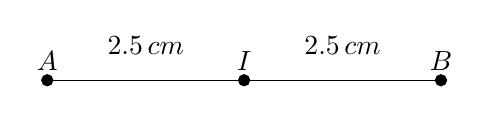
\begin{tikzpicture}
			\draw (0,0) --(5,0);
			\filldraw[black] (0,0) circle[radius = 2pt] node [above] {$A$};
			\filldraw[black] (2.5,0) circle[radius = 2pt] node [above] {$I$};
			\filldraw[black] (5,0) circle[radius = 2pt] node [above] {$B$};
			
			\draw (1.25,0.2) node [above] {$2.5\, cm$};
			\draw (3.75,0.2) node [above] {$2.5\, cm$};
		\end{tikzpicture}
	
\end{Answer}
\begin{Answer}{18}
		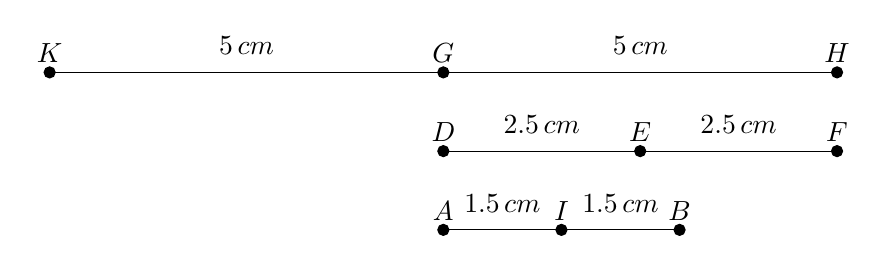
\begin{tikzpicture}
			\draw (0,0) -- (3, 0) (0,1) -- (2.5, 1) -- (5,1) (0,2) -- (5,2) (0,2) -- (-5,2);
			\filldraw[black] (0,0) circle[radius = 2pt] node[above]{$A$};
			\filldraw[black] (3,0) circle[radius = 2pt] node[above]{$B$};
			\filldraw[black] (1.5,0) circle[radius = 2pt] node[above]{$I$};
			\filldraw[black] (0,1) circle[radius = 2pt] node[above]{$D$};
			\filldraw[black] (2.5,1) circle[radius = 2pt] node[above]{$E$};
			\filldraw[black] (5,1) circle[radius = 2pt] node[above]{$F$};
			\filldraw[black] (0,2) circle[radius = 2pt] node[above]{$G$};
			\filldraw[black] (5,2) circle[radius = 2pt] node[above]{$H$};
			\filldraw[black] (-5,2) circle[radius = 2pt] node[above]{$K$};
			
			\draw (0.75,0.1) node[above]{$1.5\,cm$};
			\draw (2.25,0.1) node[above]{$1.5\,cm$};
			\draw (1.25,1.1) node[above]{$2.5\,cm$};
			\draw (3.75,1.1) node[above]{$2.5\,cm$};
			\draw (2.5,2.1) node[above]{$5\,cm$};
			\draw (-2.5,2.1)node[above]{$5\,cm$};
		\end{tikzpicture}
	
\end{Answer}
\begin{Answer}{19}
		Vì  $C$ nằm giữa $A,B$ nên ta có: $AB=AC+BC$
		
		$\Rightarrow 5=AC+3\Rightarrow AC=5-3=2$ (cm)
		
		Vì $B$ nằm giữa $A,D$ nên $AD=AB+BD$
		
		$\Rightarrow AD=5+1=6$ (cm)
	
\end{Answer}
\begin{Answer}{20}
		\begin{enumerate}[a),leftmargin=*]
			\i	Vì $A$ nằm giữa $O,B$ nên $OB=OA+AB=5+9=14\left( cm \right)$
			\begin{center}
				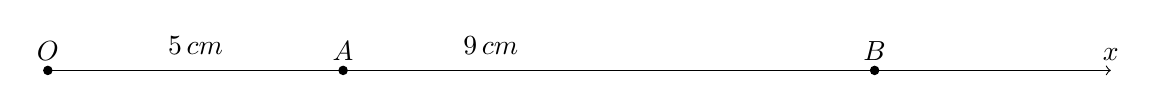
\begin{tikzpicture}[scale=0.75]
					\draw[->] (0,0) -- (18,0);
					\filldraw[black] (0,0) circle[radius = 2pt] node [above] {$O$};
					\filldraw[black] (5,0) circle[radius = 2pt] node [above] {$A$};
					\filldraw[black] (14,0) circle[radius = 2pt] node [above] {$B$};
					\draw (18,0) node[above] {$x$};		
					\draw (2.5,0.1) node[above] {$5\,cm$};		
					\draw (7.5,0.1) node[above] {$9\,cm$};						
				\end{tikzpicture}
			\end{center}
			\i TH1: $M$ nằm giữa $A,N$\\
			Ta có: $AN=AM+MN=7+2=9$ (cm)
			\begin{center}
				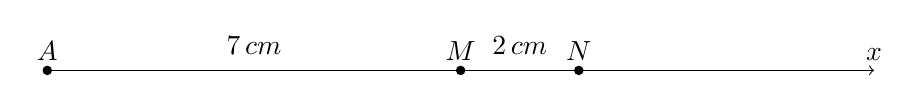
\begin{tikzpicture}[scale=0.75]
					\draw[->] (0,0) -- (14,0);
					\filldraw[black] (0,0) circle[radius = 2pt] node [above] {$A$};
					\filldraw[black] (7,0) circle[radius = 2pt] node [above] {$M$};
					\filldraw[black] (9,0) circle[radius = 2pt] node [above] {$N$};
					\draw (14,0) node[above] {$x$};		
					\draw (3.5,0.1) node[above] {$7\,cm$};		
					\draw (8,0.1) node[above] {$2\,cm$};						
				\end{tikzpicture}
			\end{center}
			TH2: $N$ nằm giữa $A,M$\\
			Ta có: $AM=AN+NM$\\
			$\Rightarrow 7 = AN + 2$\\
			$\Rightarrow AN = 7 - 2 = 5$ (cm).
		\end{enumerate}
	
\end{Answer}
\begin{Answer}{21}
		Vì $M$ thuộc đoạn thẳng $AB$  nên ta có: $AB = MB + MA$\\
		$\Rightarrow 10 = MB + MA$\\
		Mà $MB - MA = 4$\\
		Khi đó $MB = 7$ cm; $MA = 3$ cm.
	
\end{Answer}
\begin{Answer}{22}
		Vì $P$ là trung điểm của $MI$ nên ta có: $MP = IP = \dfrac{MI}{2}$\\
		$\Rightarrow MI = 2IP = 2\cdot 3 = 6$ (cm)\\
		Vì $I$ là trung điểm của $MN$ nên ta có: $MI = IN = \dfrac{MN}{2}$\\
		$\Rightarrow MN = 2MI = 2\cdot 6 = 12$ (cm)\\
		Vậy $MN = 12$ (cm)
	
\end{Answer}
\begin{Answer}{23}
		\begin{enumerate}[a),leftmargin=*]
			\i Khi sử dụng thước đo độ dài:
			\begin{enumerate}[+,leftmargin=*]
				\i Đo độ dài của bàn học và ghi chú lại số liệu
				\i Điểm chính giữa của bàn học chính là trung điểm của đoạn thẳng đo được
				\i Dựa vào số liệu đã ghi chú và áp dụng công thức tính trung điểm đoạn thẳng xác định số đo
				\i Sử dụng số đo tính toán được áp dụng lên bàn học đó là điểm chính giữa của bàn
			\end{enumerate}
			\i Khi sử dụng đoạn dây vừa đủ:
			\begin{enumerate}[+,leftmargin=*]
				\i Điểm chính giữa của bàn học là trung điểm của đoạn dây chúng ta sử dụng
				\i Gấp đôi đoạn dây lại sao cho hai đầu dây bằng nhau, đánh dấu điểm chính giữa của đoạn dây
				\i Khi đó điểm đánh dấu chính là trung điểm của đoạn dây hay cũng là điểm chính giữa của bàn học
			\end{enumerate}
		\end{enumerate}
	
\end{Answer}
\begin{Answer}{24}
		Chọn điểm $A$  trùng với điểm thấp nhất của vòng quay mặt trời (so với mặt đất)
		
		Chọn điểm $B$  trùng với điểm cao nhất của vòng quay mặt trời (so với mặt đất)
		
		Khi đó, độ đài đoạn thẳng  $AB$ là: $AB = 64-8 = 56$ (cm)
		
		Theo cách xây dựng của vòng quay mặt trời thì điểm cao nhất của trục sẽ trùng với trung điểm của đoạn thẳng  $AB$, nên trung điểm của đoạn thẳng $AB$ nằm ở độ cao là: $\dfrac{AB}{2} = \dfrac{56}{2} = 28$ (m)
		Như vậy, trục của vòng quay mặt trời sẽ nằm ở độ cao $28 + 8 = 36$ (m)
	
\end{Answer}
\begin{Answer}{25}
		Vì $P$ là trung điểm của $ON$ nên ta có: $OP = PN = \dfrac{ON}{2} = \dfrac{6}{2} = 3$ (cm)
		
		Vì $O$ nằm giữa $M,P$ và $OM=OP=3cm$ nên $O$ là trung điểm của $MP$.
	
\end{Answer}
\begin{Answer}{26}
		Vì $M$ nằm giữa $A,B$ và $AM=MB=\dfrac{AB}{2}=\dfrac{a}{2}$ nên $M$ là trung điểm của đoạn thẳng$AB$
		\begin{center}
			\begin{tikzpicture}
				\draw (0,0) -- (8,0);
				\filldraw[black] (0,0) circle[radius = 2pt] node [above] {$A$};
				\filldraw[black] (3,0) circle[radius = 2pt] node [above] {$M$};
				\filldraw[black] (6,0) circle[radius = 2pt] node [above] {$B$};
				\draw (1.5,0.1) node[above] {$\dfrac{a}{2}$};	
			\end{tikzpicture}
		\end{center}
	
\end{Answer}
\begin{Answer}{27}
		TH1:
		\begin{center}
			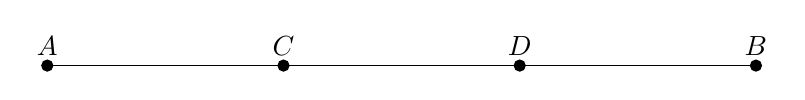
\begin{tikzpicture}
				\draw (0,0) -- (9,0);
				\filldraw[black] (0,0) circle[radius = 2pt] node [above] {$A$};
				\filldraw[black] (3,0) circle[radius = 2pt] node [above] {$C$};
				\filldraw[black] (6,0) circle[radius = 2pt] node [above] {$D$};
				\filldraw[black] (9,0) circle[radius = 2pt] node [above] {$B$};
			\end{tikzpicture}
		\end{center}
		Vì $C$ nằm giữa $A,D$ nên ta có: $AC+CD=AD$\\
		Vì $D$ nằm giữa $B,C$ nên ta có: $BC+CD=BC$\\
		Mà $AC=BD$ và $CD$ chung $\Rightarrow AD=BC$\\
		TH2:
		\begin{center}
			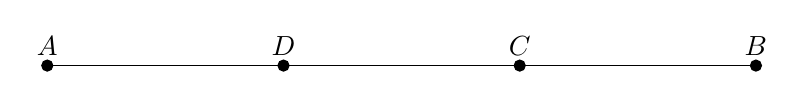
\begin{tikzpicture}
				\draw (0,0) -- (9,0);
				\filldraw[black] (0,0) circle[radius = 2pt] node [above] {$A$};
				\filldraw[black] (3,0) circle[radius = 2pt] node [above] {$D$};
				\filldraw[black] (6,0) circle[radius = 2pt] node [above] {$C$};
				\filldraw[black] (9,0) circle[radius = 2pt] node [above] {$B$};
			\end{tikzpicture}
		\end{center}
		Vì $D$ nằm giữa $A,C$ nên ta có: $AC=AD+DC\Rightarrow AD=AC-DC$\\
		Vì $C$ nằm giữa $B,D$ nên ta có: $BD=BC+DC\Rightarrow BC=BD-DC$\\
		Mà $AC=BD$ và $DC$ chung $\Rightarrow AD=BC$
	
\end{Answer}
\begin{Answer}{28}
		Vì $A$ nằm giữa $O,B$ nên ta có: $OB=OA+AB=a+b$\\
		Vì $C$ là trung điểm của $OB$ nên ta có: $OC=CB=\dfrac{OB}{2}=\dfrac{a+b}{2}$\\
		Vì $A$ nằm giữa $O,C$ nên ta có: $OC=OA+AC$\\
		\begin{center}
			\begin{tikzpicture}
				\draw (0,0) -- (13,0);
				\filldraw[black] (0,0) circle[radius = 2pt] node [above] {$O$};
				\filldraw[black] (4,0) circle[radius = 2pt] node [above] {$A$};
				\filldraw[black] (5,0) circle[radius = 2pt] node [above] {$C$};
				\filldraw[black] (9,0) circle[radius = 2pt] node [above] {$B$};
				\draw (13,0.1) node[above] {$x$};
			\end{tikzpicture}
		\end{center}
		$\Rightarrow \dfrac{a + b}{2} = a + AC$\\
		$\Rightarrow AC = \dfrac{a+b}{2} - a = \dfrac{b-a}{2}$\\
		Vậy $AC = \dfrac{b-a}{2}$
	
\end{Answer}
\begin{Answer}{29}
		Vì $A$ nằm giữa $B,C$ và $3AB=4AC$ nên ta chia $BC$ thành 7 phần bằng nhau và xác định điểm $A$ như hình vẽ.
		\begin{center}
			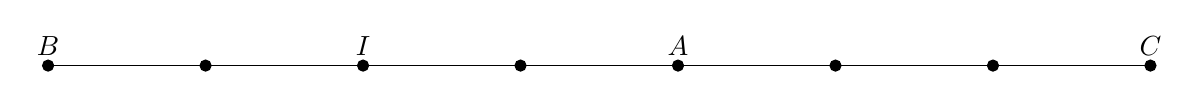
\begin{tikzpicture}
				\draw (0,0) -- (14,0);
				\filldraw[black] (0,0) circle[radius = 2pt] node [above] {$B$};
				\filldraw[black] (2,0) circle[radius = 2pt];
				\filldraw[black] (4,0) circle[radius = 2pt] node [above] {$I$};
				\filldraw[black] (6,0) circle[radius = 2pt];
				\filldraw[black] (8,0) circle[radius = 2pt] node [above] {$A$};
				\filldraw[black] (10,0) circle[radius = 2pt];
				\filldraw[black] (12,0) circle[radius = 2pt];
				\filldraw[black] (14,0) circle[radius = 2pt] node [above] {$C$};
			\end{tikzpicture}
		\end{center}
		Vì $I$ là trung điểm của $AB$ nên ta có: $BI=AI=\dfrac{AB}{2}$\\
		$\Rightarrow AI=2BI=2\cdot4=8$ (cm)\\
		Lại có: $3AB=4AC\Rightarrow AC=\dfrac{3AB}{4}=\dfrac{3\cdot8}{4}=6$ (cm)\\
		Vì $A$ nằm giữa $B,C$ nên ta có: $BC=AB+AC=8+6=14$ (cm)\\
		Vậy $BC=14$ (cm)
	
\end{Answer}
\begin{Answer}{30}
		Vì ${{A}_{1}}$ là trung điểm của $AB$ nên ta có: $A{{A}_{1}}=AB.\dfrac{1}{2}$ (m)\\
		Vì ${{A}_{2}}$ là trung điểm của $A{{A}_{1}}$ nên ta có: $A{{A}_{2}}=\dfrac{A{{A}_{1}}}{2}=AB\cdot\dfrac{1}{2}\cdot\dfrac{1}{2}$ (m)\\
		Vì ${{A}_{3}}$ là trung điểm của $A{{A}_{2}}$ nên ta có: $A{{A}_{3}}=\dfrac{A{{A}_{2}}}{2}=\dfrac{A{{A}_{1}}}{2}\cdot\dfrac{1}{2}=AB\cdot\dfrac{1}{2}\cdot\dfrac{1}{2}\cdot\dfrac{1}{2}$ (m)\\
		Vì ${{A}_{4}}$ là trung điểm của $A{{A}_{3}}$ nên ta có: $A{{A}_{4}}=\dfrac{A{{A}_{3}}}{2}=\dfrac{A{{A}_{2}}}{2}\cdot\dfrac{1}{2}=\dfrac{A{{A}_{1}}}{2}\cdot\dfrac{1}{2}\cdot\dfrac{1}{2}=AB\cdot\dfrac{1}{2}\cdot\dfrac{1}{2}\cdot\dfrac{1}{2}\cdot\dfrac{1}{2}$ (m)\\
		Như vậy, khi ta lấy trung điểm ${{A}_{n}}$ của $AB$ thì $A{{A}_{n}}=AB\cdot{{ \left(\dfrac{1}{2} \right)}^{n}}$ (m)\\
		Vậy độ dài đoạn thẳng $A{{A}_{20}}=AB.{{\left(\dfrac{1}{2} \right)}^{n}}=1\cdot{{ \left(\dfrac{1}{2} \right)}^{20}}={{\left(\dfrac{1}{2} \right)}^{20}}$ (m)
	
\end{Answer}
\begin{Answer}{31}
		Do cứ 2 điểm thì tạo thành 1 đường thẳng và không có 3 điểm nào thẳng hàng nên 10 điểm sẽ nối được với 9 điểm và mỗi đường thẳng sẽ bị trùng nên ta có:
		
		Số đường thẳng được tạo thành là: $\dfrac{10 \cdot 9}{2}=45 $ (đường thẳng)
		
		Vậy tạo thành được 45 đường thẳng khác nhau có đầu mút là 2 trong 10 điểm đã cho.
	
\end{Answer}
\begin{Answer}{32}
		Do $5AB = 8BM \Rightarrow Bm = \dfrac{5AB}{8}$\\
		Mà $Bi = \dfrac{AB}{2}$\\
		$\Rightarrow Mi = BM - BI = \dfrac{5}{8}AB - \dfrac{1}{2}AB = \dfrac{1}{8} AB$.\\
		$\Rightarrow \dfrac{1}{8} AB = 2$ (cm)\\
		$\Rightarrow AB = 16$ (cm)
	
\end{Answer}
\begin{Answer}{33}
		Vì $OA<OB$ nên $A$ nằm giữa $O$ và $B$ $\Rightarrow AB=b-a$.\\
		Vì $C$ là trung điểm của $OB$ nên $OC=CB=\dfrac{b}{2}$\\
		TH1: Nếu $a<\dfrac{b}{2}$thì $OA<OC\Rightarrow OA+AC=OC\Rightarrow AC=OC-OA=\dfrac{b}{2}-a$\\
		TH2: Nếu $a>\dfrac{b}{2}$thì $OC<OA\Rightarrow OC+AC=OA\Rightarrow AC=OA-OC=a-\dfrac{b}{2}$
		\begin{center}
			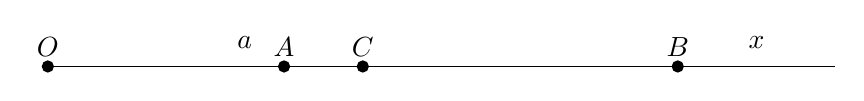
\begin{tikzpicture}
				\draw (0,0) -- (10,0);
				\filldraw[black] (0,0) circle[radius = 2pt] node [above] {$O$};
				\filldraw[black] (3,0) circle[radius = 2pt] node [above] {$A$};
				\filldraw[black] (4,0) circle[radius = 2pt] node [above] {$C$};
				\filldraw[black] (8,0) circle[radius = 2pt] node [above] {$B$};
				\draw (2.5,0.1) node[above] {$a$};
				\draw (9,0.1) node[above] {$x$};
			\end{tikzpicture}
		\end{center}
	
\end{Answer}
\begin{Answer}{34}
		Ta xét các trường hợp sau:\\
		TH1: $O$ cùng phía với 2 điểm $A,B.$
		\begin{center}
			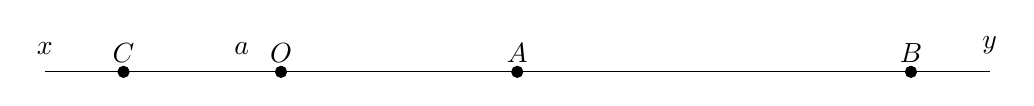
\begin{tikzpicture}
				\draw (0,0) -- (12,0);
				\filldraw[black] (1,0) circle[radius = 2pt] node [above] {$C$};
				\filldraw[black] (3,0) circle[radius = 2pt] node [above] {$O$};
				\filldraw[black] (6,0) circle[radius = 2pt] node [above] {$A$};
				\filldraw[black] (11,0) circle[radius = 2pt] node [above] {$B$};
				\draw (2.5,0.1) node[above] {$a$};
				\draw (0,0.1) node[above] {$x$};
				\draw (12,0.1) node[above] {$y$};
			\end{tikzpicture}
		\end{center}
		Do $OA=3cm$; $OB=8cm$  và $O$ cùng phía với 2 điểm $A,B$  nên $A$  nằm giữa $O$ và $B$.\\
		$\Rightarrow AB=OB-OA=8-3=5$ (cm).\\
		$A$  là trung điểm của $CB \Rightarrow C$ thuộc tia đối của tia $AB$  hay $A$  nằm giữa $C,B$ và $AC=AB=5$ (cm).\\
		$\Rightarrow AC>AO \Rightarrow O$  nằm giữa $A,C$.\\
		$\Rightarrow OC=AC-AO=5-3=2$ (cm).\\
		TH2: $O$  khác phía với 2 điểm $A,B$.\\
		\begin{center}
			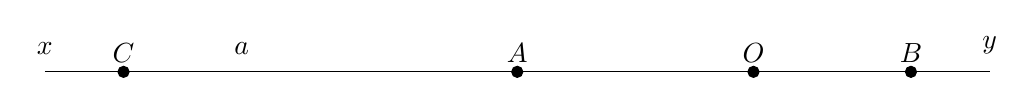
\begin{tikzpicture}
				\draw (0,0) -- (12,0);
				\filldraw[black] (1,0) circle[radius = 2pt] node [above] {$C$};
				\filldraw[black] (9,0) circle[radius = 2pt] node [above] {$O$};
				\filldraw[black] (6,0) circle[radius = 2pt] node [above] {$A$};
				\filldraw[black] (11,0) circle[radius = 2pt] node [above] {$B$};
				\draw (2.5,0.1) node[above] {$a$};
				\draw (0,0.1) node[above] {$x$};
				\draw (12,0.1) node[above] {$y$};
			\end{tikzpicture}
		\end{center}
		Do $O$  khác phía với 2 điểm $A,B$  nên $O$  nằm giữa $A$  và $B$.\\
		$\Rightarrow AB=OA+OB=3+8=11$ (cm).\\
		$A$  là trung điểm của $CB \Rightarrow C$ thuộc tia đối của tia $AB$  hay $A$  nằm giữa $C,B$ và $AC=AB=11$ (cm).\\
		$\Rightarrow A$ nằm giữa $C,O$ $\Rightarrow OC=OA+AC=3+11=14$ (cm).
	
\end{Answer}
